

\begin{frame}{Bonnes pratiques dans le numérique}{Conseils 89-90/115}
\begin{block}{Limiter l'utilisation des GIFs animés}
Le gif animé, format image animée datant de 1995, est plus lourd et plus lent que d'autres formats tels que les formats vidéo webm ou le mp4. Le webp animé est moindre dans son gain de poids et est actuellement peu supporté par les navigateurs.
\begin{figure}
    \centering
    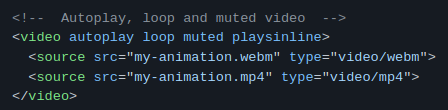
\includegraphics[scale=0.4]{chapitre2/wdd8/fig/c1.png}
\end{figure}
\end{block}

\begin{block}{Éviter la lecture/chargement automatique des vidéos/sons}L'activation automatique des vidéos et des sons au chargement des pages web implique une utilisation de ressources sur chaque tiers.

\begin{figure}
    \centering
    
\includegraphics[scale=0.4]{chapitre2/wdd8/fig/c2.png}
    
\includegraphics[scale=0.4]{chapitre2/wdd8/fig/c3.png}
\end{figure}
\end{block}
\end{frame}


\begin{frame}{Bonnes pratiques dans le numérique}{Conseils 91-93/115}
\begin{block}{Utiliser les compartiments CSS}
Le CSS Containment indique qu'un nœud et son contenu sont, autant que possible, indépendants du reste de l'arborescence de la page.
\end{block}

\begin{block}{Fournir une alternative textuelle aux contenus multimédias}

Le texte utilise beaucoup moins de bande passante que des formats multimédias comme l'audio ou la vidéo. 

\end{block}
\begin{block}{Privilégier HTTP/2 à HTTP/1}
Le protocole HTTP/2 a troqué la représentation textuelle des requêtes et réponses pour une représentation binaire avec un mécanisme de compression des entêtes HTTP (HPACK). Il permet aussi le multiplexage des échanges, permettant de n'utiliser qu'une seule connexion TCP (et donc un seul handshake TLS) avec le serveur, et ainsi tirer le meilleur avantage de HPACK.
\end{block}
\end{frame}



\begin{frame}{Bonnes pratiques dans le numérique}{Conseils 94-96/115}
\begin{block}{Économiser de la bande passante grace à un ServiceWorker}
La plupart des pages partagent une structure commune encadrant le "contenu utile". 
\end{block}

\begin{block}{Mettre en place un sitemap efficient}
Le sitemap facilite l'indexation des pages et des contenus d'un site web par les moteurs de recherche. Un sitemap non mis à jour peut contenir des urls qui n'ont plus raison d'y être car elles font référence à des pages ou des contenus peu visités et peu utiles. 
\end{block}

\begin{block}{Assurer la compatibilité avec les plus anciens appareils et logiciels du parc}
S'assurer de la compatibilité du site avec les plus anciens matériels et logiciels que les utilisateurs peuvent possèder. Les pages doivent être utilisables sur les configurations les plus contraignantes : pas de mises en page cassées, de boutons inactifs ou autre problème empêchant la lecture.
\end{block}

\end{frame}


\begin{frame}{Bonnes pratiques dans le numérique}{Conseils 97-98/115}
\begin{block}{Réduire le volume de données stockées au strict nécessaire}
Réduire le volume de données stockées par l'optimisation et la suppression.
\end{block}

\begin{block}{Utiliser une politique d'expiration/suppression des données}
 Il est obligatoire d'après le RGPD par la CNIL.
\begin{figure}
    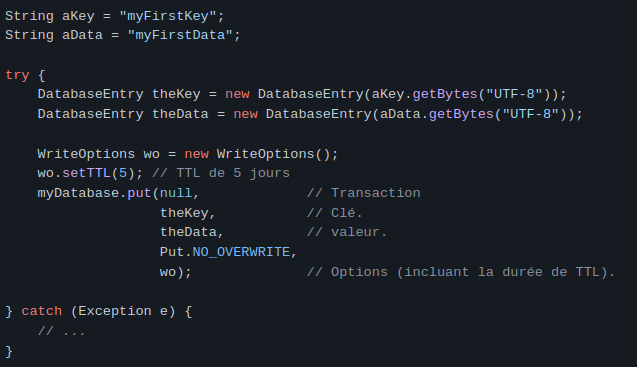
\includegraphics[scale=0.35]{chapitre2/wdd8/fig/c4.png}
\end{figure}

\end{block}


\end{frame}


\begin{frame}{Bonnes pratiques dans le numérique}{Conseils 99-101/115}
\begin{block}{Limiter le recours aux canvas}
L'élément HTML canvas est initialement conçu pour dessiner des graphiques, réaliser des jeux ou générer des images à la volée via des API JavaScript.
\end{block}

\begin{block}{S'assurer que les parcours utilisateurs permettent de réaliser leur action prévue}
Des services web permettent de réaliser sans se déplacer des démarches administratives, des ouvertures de contrats, des déclarations de sinistres etc.
\end{block}

\begin{block}{Avoir un titre de page et une metadescription pertinents avec le contenu de la page}
Un titre de page <h1>, ainsi que son équivalent <title>, adjoints à une balise <meta name="description"> pertinente doivent être parfaitement en accord avec le contenu de la page associée. 
\end{block}

\end{frame}




\begin{frame}{Bonnes pratiques dans le numérique}{Conseils 99-101/115}
\begin{block}{Limiter le recours aux canvas}
L'élément HTML canvas est initialement conçu pour dessiner des graphiques, réaliser des jeux ou générer des images à la volée via des API JavaScript.
\end{block}

\begin{block}{S'assurer que les parcours utilisateurs permettent de réaliser leur action prévue}
Des services web permettent de réaliser sans se déplacer des démarches administratives, des ouvertures de contrats, des déclarations de sinistres etc.
\end{block}

\begin{block}{Avoir un titre de page et une metadescription pertinents avec le contenu de la page}
Un titre de page <h1>, ainsi que son équivalent <title>, adjoints à une balise <meta name="description"> pertinente doivent être parfaitement en accord avec le contenu de la page associée. 
\end{block}

\end{frame}


\begin{frame}{Pause débunkage }{Nudge}
\begin{figure}
    \centering
    
\includegraphics[scale=1]{chapitre2/wdd8/fig/Nudge.jpg}
\end{figure}
\end{frame}